%%%%%%%%%%%%%%%%%%%%%%% file template.tex %%%%%%%%%%%%%%%%%%%%%%%%%
%
% This is a general template file for the LaTeX package SVJour3
% for Springer journals.          Springer Heidelberg 2010/09/16
%
% Copy it to a new file with a new name and use it as the basis
% for your article. Delete % signs as needed.
%
% This template includes a few options for different layouts and
% content for various journals. Please consult a previous issue of
% your journal as needed.
%
%%%%%%%%%%%%%%%%%%%%%%%%%%%%%%%%%%%%%%%%%%%%%%%%%%%%%%%%%%%%%%%%%%%
%
% First comes an example EPS file -- just ignore it and
% proceed on the \documentclass line
% your LaTeX will extract the file if required
\begin{filecontents*}{example.eps}
%!PS-Adobe-3.0 EPSF-3.0
%%BoundingBox: 19 19 221 221
%%CreationDate: Mon Sep 29 1997
%%Creator: programmed by hand (JK)
%%EndComments
gsave
newpath
  20 20 moveto
  20 220 lineto
  220 220 lineto
  220 20 lineto
closepath
2 setlinewidth
gsave
  .4 setgray fill
grestore
stroke
grestore
\end{filecontents*}
%
\RequirePackage{fix-cm}
%
%\documentclass{svjour3}                     % onecolumn (standard format)
%\documentclass[smallcondensed]{svjour3}     % onecolumn (ditto)
%\documentclass[smallextended]{svjour3}       % onecolumn (second format)
\documentclass[twocolumn]{svjour3}          % twocolumn
%
\smartqed  % flush right qed marks, e.g. at end of proof
%
\usepackage{graphicx}
\usepackage{amsmath}
\usepackage{subfigure}
%\usepackage[square]{natbib}
%
% \usepackage{mathptmx}      % use Times fonts if available on your TeX system
%
% insert here the call for the packages your document requires
%\usepackage{latexsym}
% etc.
%
% please place your own definitions here and don't use \def but
% \newcommand{}{}
%
% Insert the name of "your journal" with
% \journalname{myjournal}
%
\begin{document}

\title{Lazy Shadowing%\thanks{Grants or other notes
%about the article that should go on the front page should be
%placed here. General acknowledgments should be placed at the end of the article.}
}
\subtitle{An Energy-Aware Resilience Approach for High Performance Computing}

%\titlerunning{Short form of title}        % if too long for running head

\author{Xiaolong Cui         \and
        Bryan Mills          \and
        Taieb Znati          \and
        Rami Melhem
}

%\authorrunning{Short form of author list} % if too long for running head

\institute{Xiaolong Cui \at
              University of Pittsburgh, U.S. \\
              \email{mclarencui@cs.pitt.edu}           %  \\
%             \emph{Present address:} of F. Author  %  if needed
           \and
           Bryan Mills \at
              University of Pittsburgh, U.S. \\
              \email{bmills@cs.pitt.edu}
          \and
           Taieb Znati \at
              University of Pittsburgh, U.S. \\
              \email{znati@cs.pitt.edu}
          \and
           Rami Melhem \at
              University of Pittsburgh, U.S. \\
              \email{melhem@cs.pitt.edu}
}

\date{Received: date / Accepted: date}
% The correct dates will be entered by the editor


\maketitle

\begin{abstract}
With the concerted efforts from researchers in hardware, software, algorithm, and data management, HPC is moving towards extreme-scale, featuring a computing capability of quintillion ($10^{18}$) FLOPS. 
As we approach the new era of computing, however, several daunting scalability challenges remain to be conquered. Delivering extreme-scale performance will require a computing platform that supports billion-way parallelism, necessitating a dramatic increase in the number of computing, storage, and networking components. At such a large scale, failure would become a norm rather than an exception, driving the system to significantly lower efficiency with unprecedented amount of power consumption. %The frequency and diversity of failures,  as well as the challenge of power, call for rethinking of the fault tolerance problem. 

To tackle this challeng, we propose an adaptive and power-aware algorithm, referred to as Lazy Shadowing, as an efficient and scalable approach to achieve high-levels of resilience, through forward progress, in extreme-scale, failure-prone computing environments. 
Lazy Shadowing associates with each process a ``shadow" (process) that executes at a reduced rate, and opportunistically rolls forward each shadow to catch up with the its leading process during failure recovery.
%overlaps the recovery time after each failure with the time needed to roll forward the shadows to a consistent state.
Compared to existing fault tolerance methods, our approach can achieve 20\% energy saving with potential reduction in solution time at scale.

\keywords{Fault Tolerance \and Lazy Shadowing \and Energy Awareness}
% \PACS{PACS code1 \and PACS code2 \and more}
% \subclass{MSC code1 \and MSC code2 \and more}
\end{abstract}

\section{Introduction}
\label{intro}
As our reliance on information technology continues to increase, the complexity and urgency of the problems our society will face in the future will increase much faster than are our abilities to understand and deal with them. It is expected that in the future, increasingly more complex applications will require very high computing performance and will process massive volume of data. Addressing these challenges requires radical changes in the way computing is delivered to support the computing requirements of these applications~\cite{sachs_ascr_2011}. New algorithms and programming models must be developed to enable significantly higher levels of parallelism. It is expected that the number of concurrent threads to sustain these required levels of parallelism will rise to a billion, a factor of 10,000 greater than what current platforms can support. This in turn will result in a massive increase in the number of computing cores, memory modules and storage components.

A direct implication of these emerging trends is the need to address the difficult challenge of minimizing energy consumption. Furthermore, the fault rates are expected to dramatically increase, possibly by several orders of magnitude~\cite{srinivasan_dsn_2004,torrellas2009architectures}. Figure~\ref{fig:sandia_system_mtbf} shows the system Mean Time Between Failures (MTBF) and the number of faults as a function of the number of nodes in the system~\cite{riesen_sandia_2010}. These faults, which can be transient, temporary, intermittent or permanent, stem from different causes and produce different effects. Concern about the increase of fault rates will not only be caused by the explosive growth in the number of computing and storage components, but will also grow out of the necessity to use advanced technology, operate at lower voltage levels, and deal with undesirable aging effects as they become significant~\cite{plank1995compressed}. Addressing this concern brings about unprecedented resilience challenges, which puts in question the ability of next generation HPC infrastructure to continue operation in the presence of faults without compromising the requirements of the supported applications. 


\begin{figure}[!t]
\begin{center}
	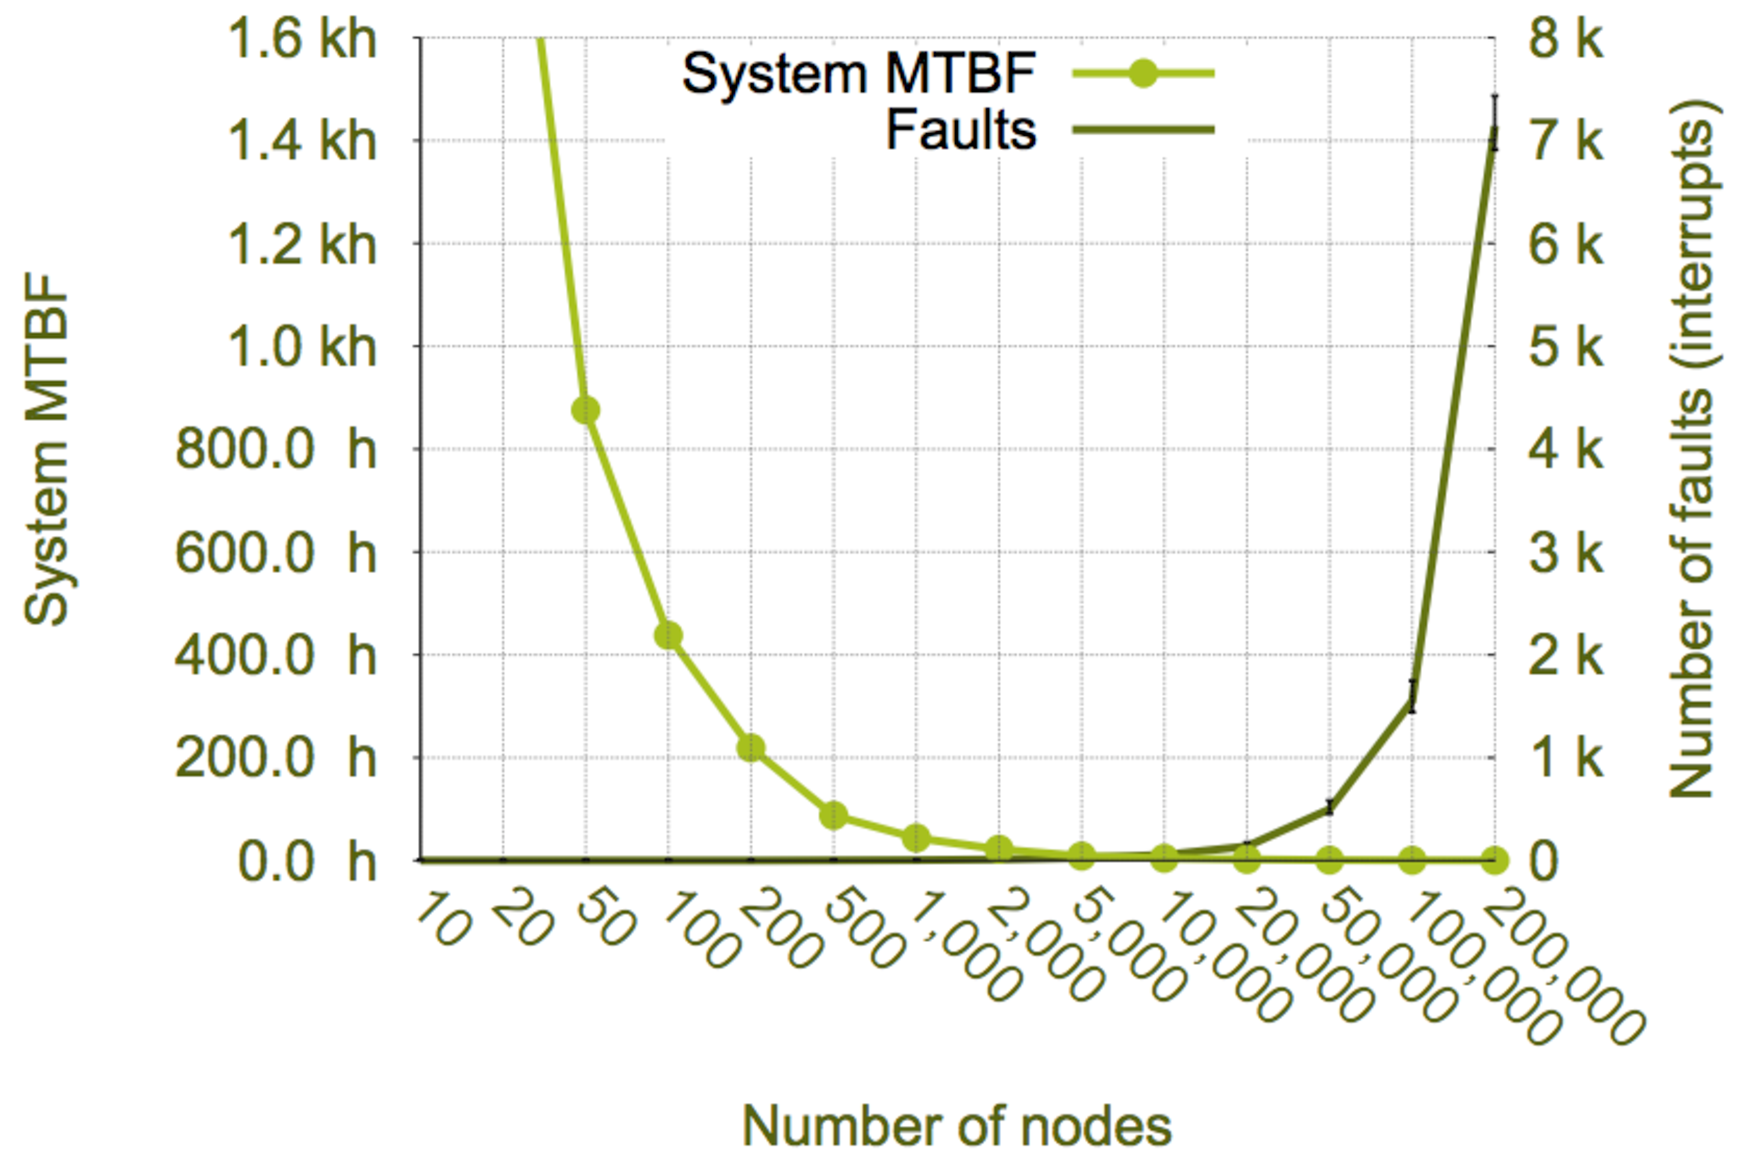
\includegraphics[width=\columnwidth]{figures/sandia_system_failure_rate_increase_nodes.pdf}
%\psfig{figure=diagrams/sandia_system_failure_rate_increase_nodes.eps,width=3.0in}
	\caption { Effect on system MTBF as number of nodes increase. }
	\label{fig:sandia_system_mtbf}
\end{center}
\end{figure}

The current response to faults consists of restarting the execution of
the application, including those components of its software
environment that have been affected by the occurring fault. To avoid
the full re-execution of the failing application, fault-tolerant
techniques typically checkpoint the execution periodically; upon the
occurrence of a hardware or software failure, recovery is achieved by
restarting the computation from a safe checkpoint. In some situations,
however, several components of the software environment associated
with the failed application may have to be restarted.

Given the anticipated increase in failure rate and the time required
to checkpoint large-scale compute- and data-intensive applications, it
is very likely that the time required to periodically checkpoint an
application and restart it upon failure may exceed the mean time
between failures.  Consequently, applications may achieve very little
computing progress, thereby reducing considerably the overall
performance of the system.  For example, a study carried out at Sandia
National Laboratories focused on evaluating the overhead incurred by
checkpointing. The results of the
study, depicted in Figure \ref{sandia_checkpoint_time}, clearly show
that beyond 50,000 nodes the application spends only a fraction of the
elapsed time performing useful computation.

\begin{figure}[!t]
\centering
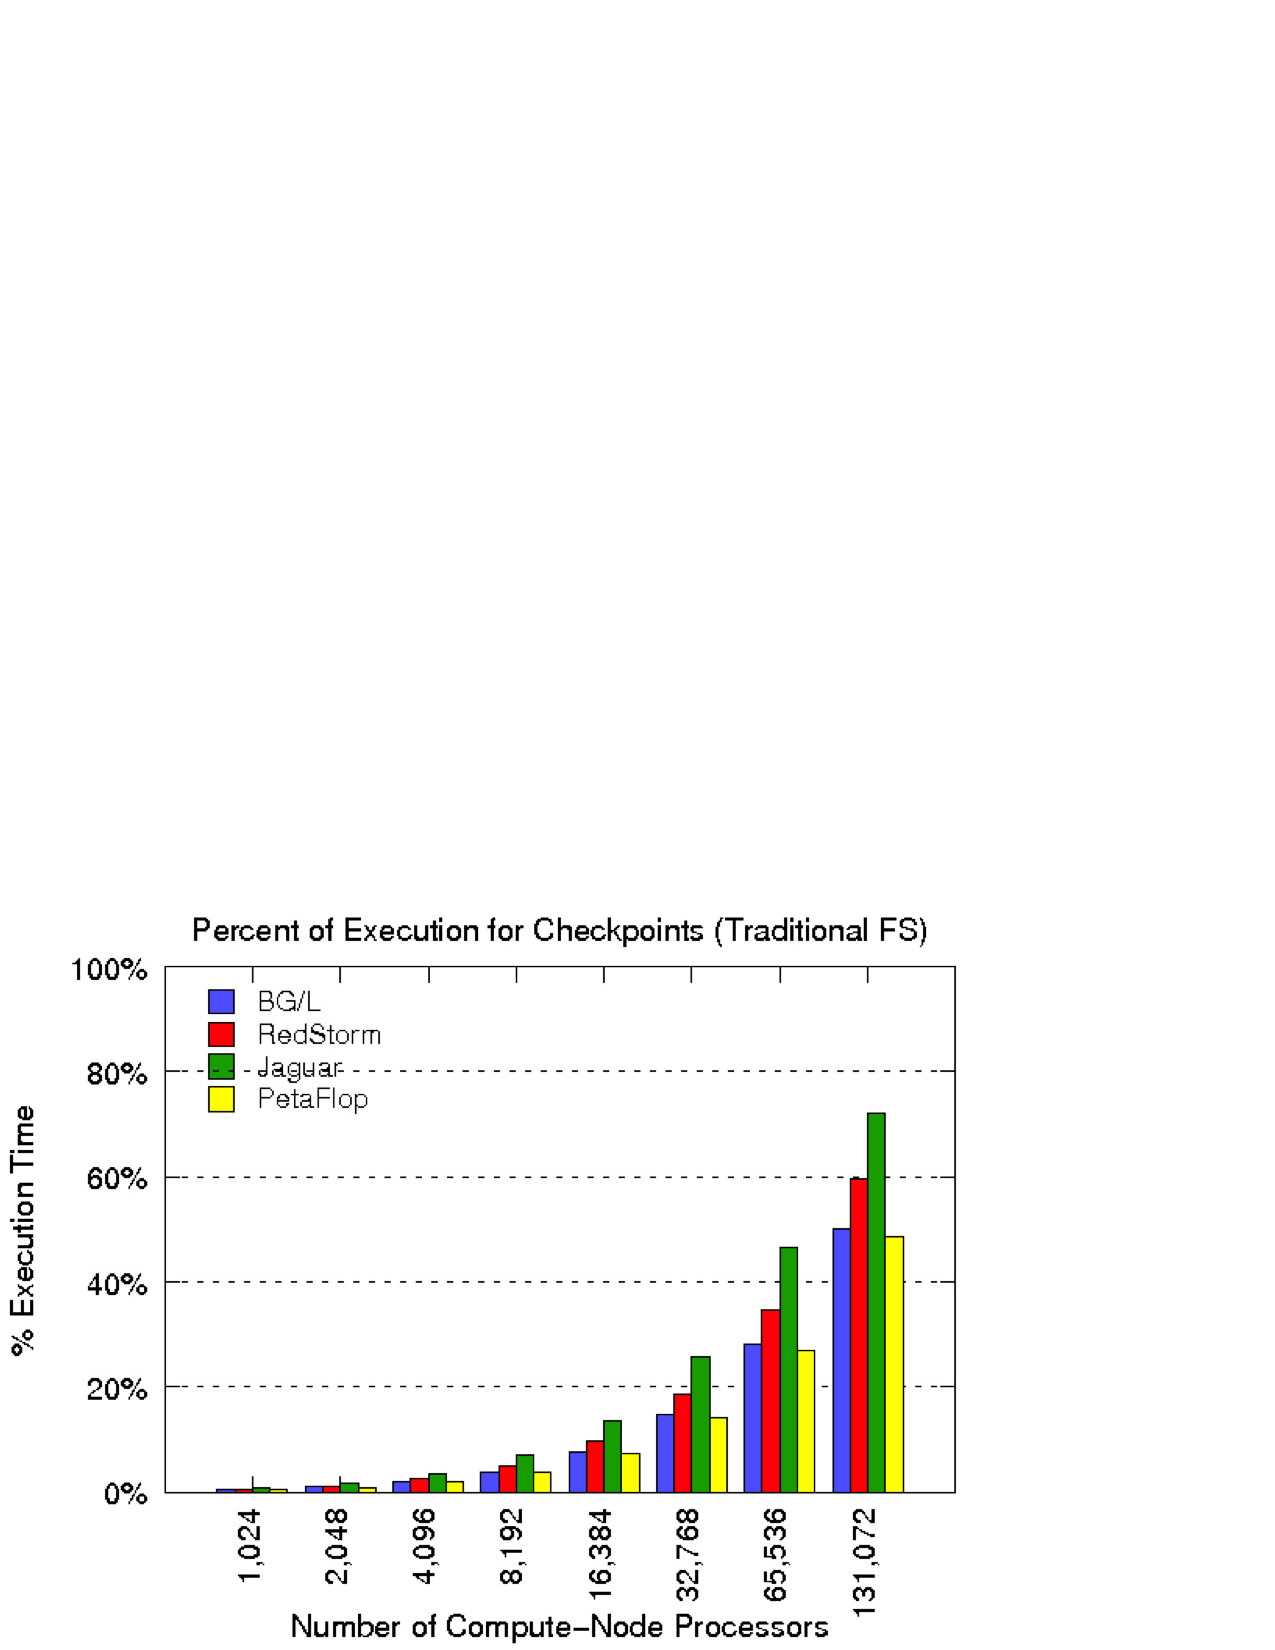
\includegraphics[width=\columnwidth]{figures/sandia_percent_of_time_for_checkpoints.pdf}
%\psfig{figure=diagrams/sandia_percent_of_time_for_checkpoints.eps,width=3.0in}
\caption { Percent of time to perform checkpoints. }
\label{sandia_checkpoint_time}
\end{figure}

%Current fault-tolerant frameworks are typically designed to handle single errors, whereas computation in large-scale, high-performance computing environments is likely to face multiple different types of errors, often concurrently. Even in the case of single errors, 
In addition, current fault-tolerant approaches apply the same technique, mainly checkpoint-restart over the entire duration of the execution, to handle all types of faults, including permanent node crashes, transient computing errors, and IO device failures. The nature of errors in large-scale, high-performance computing environments, however, are such that a general and expensive fault-tolerance technique, such as checkpoint-restart, may not be an adequate approach to handle the diverse types of faults in these environments. 

The main objective of this paper is to explore radically different
paradigms to enable scalable resiliency with minimum energy
consumption in future large-scale, high-performance computing environments. To this
end, we propose a new energy-aware ``lazy shadowing'' model, %as the
%basis for an efficient and scalable computational framework to achieve
%desired levels of fault tolerance, while minimizing energy
%consumption. The proposed model 
which goes beyond traditional checkpointing
and roll-back recovery techniques and uses a multi-level,
energy-aware replication approach to achieve scalable fault tolerance.

The basic idea of the lazy shadowing model is to associate with each
process a suite of ``shadow processes'', whose size depends on the
``criticality'' and performance requirements of the underlying
application. A shadow is an exact replica of the main process. In
order to overcome failure, the shadows are scheduled to execute
concurrently with the main process, but at different computing
nodes. Furthermore, in order to minimize energy, shadow processes
initially execute at decreasingly lower processor speeds. The
successful completion of the main process results in the immediate
termination of all shadow processes. If the main process fails, however,
the primary shadow process immediately takes over the role of the main
process and resumes computation, possibly at an increased speed, in
order to complete the task within the targeted response time. Moreover, one among the remaining shadow processes
becomes the primary shadow process.

In order to fully harness the potential of lazy shadowing to efficiently deal with failures, an optimization model is proposed to derive the execution rates of the main process and the prior- and post-failure execution rates of the shadow processes. The derived execution rates are such that the energy consumption is minimized, without violating the performance requirements of the underlying application. It is worth noting that the interplay between resilience and energy management manifests itself in different ways and must be analyzed carefully. Operating at lower voltage thresholds, for example, reduces power consumption but have adverse impact on the resilience of the system to handle high error rates in a timely and reliable fashion. Our approach will seek to avoid continuous change in voltage and frequency to prevent potential thermal and mechanical stresses on the electronic chips and board-level electrical connections. 

The remainder of the paper is organized as follows: Section
\ref{related_work} reviews work related to fault-tolerance in
large-scale high-performance computing systems. Section
\ref{model} presents the lazy shadowing framework and formulates an energy optimization problem
to achieve fault-tolerance, while minimizing energy consumption
without violating the expected performance requirements of the
supported application. In Section~\ref{application_to_hpc} two different approaches to
solving the energy optimization problem and their potential
implementation are explored. The methods differ in their approach to
energy minimization and their reaction to failures. In Section
\ref{analysis}, we develop a performance evaluation framework to
analyze and assess the performance of the three lazy shadowing
methods, including their sensitivity to critical workload and
performance parameters.  Throughout the study, the performance of the
two methods is compared to state machine replication, a recently proposed
alternative to check-pointing in large-scale HPC.  Section
\ref{conclusion} presents the conclusion of this work and discusses
future work.

\section{Related Work}
\label{related_work}
%Extreme-scale computing presents some unique challenges to fault tolerance as faults are no longer 
%an exceptional event \cite{ferreira_sc_2011}. 
Rollback and recovery is the predominate mechanism to achieve fault
tolerance in current HPC environments. In the most general form, rollback and recovery 
involves the periodic saving of the current system state, with the anticipation that
in the case of a failure, computation can be restarted from the most recently saved state \cite{Elnozahy:02:Survey}. %The identification of an error, before or during a checkpoint,
%requires that the application rollback to the previously completed checkpoint. 
Coordinated checkpointing is a popular approach for
its ease of implementation.
%Specifically, all processes
%coordinate with one another to produce individual states that satisfy the ``happens before"
%communication relationship \cite{chandy_trans_1972}, which is proved to provide a consistent global state.
%Essentially, the algorithm provides a method for all processes involved to stop operation ``at the same
%time" and transfer their system state to a stable storage. 
%The major benefit of coordinated
%checkpointing stems from its simplicity and ease of implementation. 
Its major drawback, however, is the
lack of scalability, as it requires global coordination
\cite{elnozahy_dsc_2004,riesen_sandia_2010}.
%hargrove2006berkeley}.


In uncoordinated checkpointing, processes record their states independently and postpone creating a 
globally consistent view until the recovery phase. The major advantage is the reduced overhead during fault free operation. However, the scheme requires that
each process maintains multiple checkpoints and message logs, necessary to construct a consistent 
state during recovery. It can also suffer the well-known domino effect 
 \cite{randell_domino_effect}. One hybrid approach, known as communication induced 
checkpointing, aims at reducing coordination overhead \cite{alvisi_ftc_1999}. The approach, however, may 
cause processes to store useless states. To address this 
shortcoming, ``forced checkpoints" have been proposed \cite{helary_rds_1997}. This approach, however,  may lead to unpredictable
checkpointing rates. Although well-explored, uncoordinated checkpointing has not been widely adopted
in HPC environments, due to its dependency on applications \cite{guermouche_2011_ipdps}.


One of the largest overheads in any checkpointing process is the time necessary to write the checkpointing 
to stable storage. Incremental checkpointing attempts
to address this by only writing the changes since previous checkpoint \cite{Agarwal:04:Adaptive,elnozahy_1992_manetho,li_trans_1994}. %This
%can be achieved using dirty-bit page flags \cite{plank_ftcs_1994,elnozahy_1992_manetho}. Hash based incremental checkpointing, on the other
%hand, makes use of hashes to detect changes \cite{nam_ftc_1997,Agarwal:04:Adaptive}. 
Another proposed scheme, known as in-memory checkpointing, minimizes the overhead of disk access~\cite{zheng_2004_ftccharm}.
%offloads the checkpointing process to a secondary task and only writes incremental checkpoints \cite{li_trans_1994}.
The main concern of these techniques is the increase in
memory requirement to support the simultaneous execution of the checkpointing and the application. It has been suggested that nodes in extreme-scale systems should be configured with fast local storage~\cite{doe_ascr_exascale_2011}. 
%, which
%improves the performance of checkpointing \cite{doe_ascr_exascale_2011}. 
Multi-level checkpointing, which consists of
writing checkpoints to multiple storage targets, can benefit from such a strategy \cite{Moody:10:SCR}. This,
however, may lead to increased failure rates of individual nodes and complicate the checkpoint writing process.
%Furthermore, it may complicate the checkpoint writing process and requires that the system track the
%current location of all process's checkpoints.


Our work is based on process replication, or state machine replication, which has long been used to provide fault tolerance in distributed and mission critical systems\cite{schneider_1990_tutorial}. %Replication can be used to detect and correct system failures that are otherwise undetectable,
%such as silent data corruption and Byzantine faults \cite{fiala_2012_sdc}. 
Recently, replication has been proposed as a
viable alternative to checkpointing in HPC \cite{ferreira_sc_2011,Cappello:09:Fault,fiala_2012_sdc}. 
In addition, full and partial
replication have also been used to augment existing checkpointing techniques, and to guard
against silent data corruption \cite{stearly_2012_partial,elliott_2012_cpr}.% There are several different implementations of
%replication in the widely used MPI library, each with their different tradeoffs and overheads. The
%overhead can be negligible or up to 70\% depending upon the communication patterns of the
%application \cite{engelmann2011redundant}. %Moreover, replication alone is not enough to guarantee fault tolerance since
%it is possible that all nodes executing a given process could fail simultaneously, thus
%replication is typically paired with some form of checkpointing. 
The most relevant works to ours is redundant multi-threading (RMT) whereby one leading thread of execution is running ahead of trailing threads \cite{reinhardt2000transient,Wadden:2014:RDE:2665671.2665686}. However, our approach is different in that it tunes the execution rates of the leading and trailing threads in a finer grain, in order to achieve a ``parameterized" trade-off between completion time and energy consumption. Further, we take advantage of the idle time during failure recovery and ``leap" the trailing threads to achieve forward progress%, largely improving performance in terms of both completion time and energy consumption. 
. This differs from RMT, of which the ``leaping" of the trailing thread results in extra overhead.
%To the best of our knowledge,
%Lazy Shadowing is the first attempt to explore a state-machine replication based framework
%that achieves a fine-grained tradeoff between time and hardware redundancy while meeting resilience and
%power requirements.


%\section{Model and Data Structure}
%\label{shadow_model}
%
In this section, we provide an overview of the shadow computing
execution model, under different failure scenarios. We also discuss
the mapping of the processes to the computing infrastructure to ensure
fault-tolerance to failure. Finally, we present the basic data
structure that enables efficient communication between a main process
and its associated shadow. The main purpose of this section is to show
the feasibility of the shadow computing model. The details of how the
execution model and its associated data structure are implemented is
outside the scope of this work, and will be the subject of a future
publication.


\subsection{Execution Model} 

Depending on the occurrence of failure during execution, two scenarios
are possible. The first scenario, depicted in Figure
\ref{simple_shadow_no_failure}, takes place when no failure
occurs\footnote{For the purpose of this discussion, only a single
shadow is considered. The discussion can be easily extended to deal
with multiple shadow processes}. In this scenario, the main process
executes at the optimum processor speed, namely the speed necessary to
achieve the desired level of fault-tolerance, minimize energy
consumption and meet the target response time of the supported
application. The figure shows the completion time of the task, in the
absence of failure. During this time, the main process completes the
total amount of work required by the underlying application. However,
the shadow process, executing at a reduced processor speed, only
completes a significantly smaller amount of the original workload.
Because the likelihood of an individual node failure is low, this
scenario is most likely to occur with high frequency, resulting in a
relatively small amount of additional energy consumption to achieve
fault-tolerance. The benefits of this scheme clearly outweigh the
additional energy cost. Furthermore, it is worth noting that the
failure of the shadow process does not impact the behavior of the main
process.

\begin{figure}[hHtb]
\centering
\subfigure[Shadow Computing \-\- Case of no failure]{
\label{simple_shadow_no_failure}
\psfig{figure=diagrams/shadow_simple_no_failure_work.eps,width=3.1in}
}
\subfigure[Shadow Computing \-\- Case of failure]{
\label{simple_shadow_with_failure}
\psfig{figure=diagrams/shadow_simple_with_failure_work.eps,width=3.1in}
}
\end{figure}

The second scenario, depicted in Figure
\ref{simple_shadow_with_failure}, takes place when failure of the main
process occurs. Upon failure detection, the shadow process increases
its processor speed and executes until completion of the task.  The
processor speed at which the shadow executes after failure is derived
so that the shadow computing model guarantees that the task still
completes by the targeted response time,regardless of when the failure
occurs. Furthermore, shadow computing achieves considerable energy
saving by taking advantage of the fact that the likelihood of
individual component failures in exascale computing is small, thereby
making oblivious the need to execute "duplicate work" unless a failure
occurs. It is assumed that shadow processes can detect failures
although the details of this are beyond the scope of this paper.


It is worth noting that the interplay between resiliency and power
management manifests itself in different ways and must be analyzed
carefully. Operating at lower voltage thresholds, for example, reduces
power consumption but has an adverse impact on the resiliency of the
system to handling high error rates in a timely fashion. Our approach
to deriving optimal execution speed for the main process and its
associated shadows, both before and after failure, seeks to avoid
continuous change in voltage and frequency to prevent potential
thermal and mechanical stresses on the electronic chips and
board-level electrical connections.


% LocalWords: mtbf megawatts exascale gigawatts pre varela
\subsection{Process Mapping}

In the shadow computing model the execution of a task spawns the
creation of both a main process and a suite of shadow processes. These
processes must be carefully mapped to the computing nodes of the
exascale computing infrastructure to achieve fault-tolerant execution.
Consequently, the mapping must be done such that the main and shadow
processes are {\it fault-isolated} from each other, meaning that a
fault affecting one process does not affect the other. Fault-isolation
is necessary to minimize the likelihood that both the main and shadow
processes fail at the same time. In clound computing, fault-isolation
uses the virtual computing capabilities of the infrastructure to
assign main processes and shadows in a way such a given shadow process
can only be run along side an unrelated main process.  Figure
\ref{process_allocation_diagram} illustrates a feasible assignment
that satisfies such a constraint, for the case of three main processes
and their associated shadows.

\begin{figure}[hHtb]
\centering
\psfig{figure=diagrams/overview_architecture.eps,width=3.0in}
\caption { Example Process Mapping }
\label{process_allocation_diagram}
\end{figure}

\subsection{Message Passing}

Another important aspect of the shadow computing model is providing
process communication to achieve synchronization and maintain system
consistency.  A communication model to ensure these requirements must
at a minimum support these two properties:
\begin{itemize}
\item
All messages destined for a task must be delivered to both the main
process and all associated shadow processes.
\item
Any message previously sent from a task must not be duplicated by any
of the running process.
\end{itemize}

To satisfy the communication and synchronization requirements the
shadow computing model, the runtime support environment uses a Global
Message Queue, see Figure \ref{process_allocation_diagram}. All
inter-task communication will occur through a virtual message queue,
which is assumed to be resilient to system faults. When a task spawns
the main and shadow processes the queue is notified of all processes
created. For scalability reasons we assume the queue is a {\it
passive-queue}, meaning it only stores messages and waits for them to
be requested as opposed to forwarding messages to processes. This
eliminates the need for the queue to notify processes directly and
instead lets the processes request them when they are ready. This
allows processes running at a higher execution speed to not interfere
with the execution of processes running slower.

When a message arrives at the queue for delivery to a task it will
hold that message until it has been delivered to all associated
processes\footnote{Any implementation of such a system will have to
address the issue of growing queue size but for this discussion it is
assumed we have an infinite queue.}. This is possible because all
associated processes were registered with the queue when created. An
example of message delivery is depicted in Figure
\ref{queue_message_delivery}. While not depicted, messages would also
also be removed from the queue once the task was completed. This
scheme ensures that all executing processes will receive all messages
destined for the task.

\begin{figure}[hHtb]
\centering
\psfig{figure=diagrams/message_queue_deliever.eps,width=3.0in}
\caption { Example Message Delivery }
\label{queue_message_delivery}
\end{figure}

\begin{figure}[hHtb]
\centering
\psfig{figure=diagrams/message_queue_receive.eps,width=3.0in}
\caption { Example Message Receiving }
\label{queue_message_receiving}
\end{figure}

In order to ensure that messages are not duplicated by shadow
processes we propose that all messages be assigned a unique sequence
number per task. When the queue receives a message from a task it will
determine if that message has already been received by the queue for
the task. If the message is a duplicate it will simply ignore the
message, if however it is a new message it will queued for
delivery. We show an example of the message receiving process in
Figure \ref{queue_message_receiving}. This allows shadow processes to execute
slower and not produce duplicate system messages. The other benefit of
this model is that messages will be processed regardless of their
source, therefore the queue doesn't need to be aware of process
failures.


\section{Energy Optimization Model}
\label{model}
As stated previously, the basic idea of shadow computing is to
associate a number of ``shadow processes'' with each main process. The
main responsibility of a shadow process is to take over the
responsibility of a failed main process and bring the computation to a
successful completion.  In this section, we define a framework for
evaluating shadow computing and then use this to derive a model for
representing the expected energy consumed by the system. %We then
%describe in terms of this model three different methods for applying
%shadow computing in a high performance computing environment.

%%model that describes and show how it can be used to derive the speed
%%of execution of the shadow process that minimizes energy
%%consumption. Without loss of generality, in this section, we focus on
%%the main process and its first shadow. The model can be easily
%%extended to deal with multiple shadows.

\subsection{Shadow Computing Framework}
\label{shadow_computing_framework}

We consider a distributed computing environment executing an
application composed of a large number of collaborative tasks. The
successful execution of the application depends on the successful
completion of all of these tasks. Therefore the failure of a single
process delays the entire application, increasing the need for fault
tolerance. Each task must complete a specified amount of work, $W$, by
a targeted response time, $R$. The amount of work is expressed in
terms of the number of cycles required to complete the task. Each
computing node has a variable speed, $\sigma$, given in cycles per
second and bounded such that $0\leq\sigma\leq\sigma_{max}$. Therefore
the minimum response time for a given task is $R_{min}=W/\sigma_{max}$.

In order to achieve our desired fault tolerance a shadow process
executes in parallel with the main process on a different computing
node. The main process executes at a single execution speed denoted as
$\sigma_m$. In contrast the shadow process executes at two different
speeds, a speed before failure detection, $\sigma_b$, and a speed
after failure detection, $\sigma_a$. This is depicted in Figure
\ref{shadow_overview}.

\begin{figure}[hHtb]
\centering
\psfig{figure=diagrams/shadow_main_diagram.eps,width=3.5in}
\caption { Overview of Shadow Computing }
\label{shadow_overview}
\end{figure}


\subsection{Power Model}
\label{power_model}
Dynamic voltage and frequency scaling
(DVFS) has
been widely exploited as a technique to reduce CPU dynamic power~\cite{flautner_2002_APS,pillai_2001_sosp}.
It is well known that by varying the execution speed of the computing
nodes one can reduce their dynamic power consumption at least quadratically by
reducing their execution speed linearly. The power consumption of a
computing node executing at speed $\sigma$ is given by the function
$p_d(\sigma)$, represented by a polynomial of at least second degree,
$p_d(\sigma)=\sigma^n$ where $n\geq2$. 
In addition to the dynamic power, CPU leakage and other components
(memory, disk, network etc.) all contribute to static power
consumption, which is constant as long as the system is on. In this paper we
use $\rho$ to represent the weight of static power and $1-\rho$ the weight 
of dynamic power, when the node is running at the maximum speed.
Therefore, the power consumption is expressed as $p(\sigma)=\rho \times \sigma_{max}^n + (1-\rho)\times \sigma^n$.
The energy consumed by a
computing node executing at speed $\sigma$ during an interval of
length $T$ is given by $E(\sigma,T)=\int_{t=0}^T
p(\sigma)dt$. For an interval during which the speed is constant, the 
energy consumption can be calculated as $p(\sigma)t$. Throughout this paper
we assume that dynamic power is cubic in relation to speed, i.e., 
$p(\sigma)=\rho \times \sigma_{max}^3 + (1-\rho)\times \sigma^3$
We further assume that the computing node speed is bounded by the
following equation $0\leq\sigma\leq\sigma_{max}$.

\subsection{Failure Model}
\label{failure_model}

The failure can occur at any point during the execution of the main
task and the completed work is unrecoverable. Because the processes
are executing on different computing nodes we assume failures are
independent events. We also assume that only a single failure can
occur during the execution of a task. If the main task fails it is
therefore implied that the shadow will complete without failure. We
can make this assumption because we know the failure of any one node
is a rare event thus the failure of any two specific nodes is very
unlikely. In order to achieve higher resiliency one
would make use of multiple shadow processes and this failure model
will still be valid.

We assume that a probability density function, $f(t)$ ($\int_0^\infty
f(t)dt=1$), exists which expresses the probability of the main task
failing at time $t$. 
It is worth noting, that the lazy shadowing computation model 
does not depend on any specific distribution. However, in the remainder of this 
paper we use an exponential probability density function, $f(t) = \lambda e^{-\lambda t}$.
Numerous works have
studied the impact of DVFS on the failure rate or soft error rate
~\cite{firouzi2010reliability,zhu2004effects}. To take this effect into consideration,
we adopt the most widely used model from~\cite{zhu2004effects} and expressed it
within our framework as $\lambda(\sigma) = \lambda_0 10^{1-\sigma/\sigma_{max}}$. 
%Therefore, the failure distribution function is $f(\sigma, t) =  



\subsection{Energy Model}
\label{energy_model}

Given the power model and the failure distribution, the expected
energy consumed by a shadow computing task can be derived as the weighted
average considering all possible cases. 
First consider the case where no failure occurs and the main process
successfully completes the task at time $t_c^m$.
\begin{equation}
\begin{split}
E_1 = &  ( 1-\int_0^{t_c^m}f_m(t)dt) \times (1 - \int_0^{t_c^m} f_s(t)dt) \times \\
      &  (  E(\sigma_m,t_c^m) + E(\sigma_b,t_c^m))
\label{eq:energy_no_failure}
\end{split}
\end{equation}
The first line is the probability of fault-free execution of the main
process and shadow process. Then we multiple this probablity by the
energy consumed by the main and the shadow process during this fault
free execution, ending at $t_c^m$.

Next, consider the case where the shadow process fails at some point
before the main process successfully completes the task.
\begin{equation}
\begin{split}
E_2 = & (1-\int_0^{t_c^m}f_m(t)dt) \times \\
      & \int_0^{t_c^m}(E(\sigma_m,t_c^m)+E(\sigma_b,t)) \times f_s(t)dt
\label{eq:energy_shadow_fail}
\end{split}
\end{equation}
The first factor is the probability that the main process does not
fail, and the probability of shadow fails is included in the second factor which also contains the energy consumption since it depends on the shadow failure time. Energy consumption comes from the main process until the completion of the task,
and the shadow process before its failure.

The one remaining case to consider is when the main process fails and
the shadow process must continue to process until the task completes.
\begin{equation}
\begin{split}
E_3 = & (1-\int_0^{t_c^m}f_s(t)dt) \times \int_0^{t_c^m}(E(\sigma_m,t)+\\
      & E(\sigma_b,t)+E(\sigma_a,t_c^s-t))f_m(t)dt
\label{eq:energy_main_fail}
\end{split}
\end{equation}
Similarly, the first factor expresses the probability that the shadow process does
not fail. In this case, the shadow process executes from the beginning to
$t_c^s$ when it completes the task. However, under our ``at most one
failure'' assumption, the period during which shadow process may fail
ends at $t_c^m$, since the only reason why shadow process is still in
execution after $t_c^m$ is that main process has already failed. There
are three parts of energy consumption, including that of main process
before main's failure, that of shadow process before main's failure,
and that of shadow process after main's failure, all of which depend
on the failure occurrence time. 

By summing these three parts we will have
the expected energy consumed by shadow computing for completing a
task.
\begin{equation}
E[\text{energy}]= (E_1 + E_2 + E_3)
\label{eq:total_energy}
\end{equation}

\subsection{Optimization problem formulation}\

Using the models above we formulate our objective as the following
optimization problem.
%%% need more horizontal spacing here... not sure the latex-fu
\begin{equation}
\label{optimization_problem}
%\setlength{\abovedisplayskip}{14pt}
\begin{alignedat}{2}
\min_{\sigma_m,\sigma_b,\sigma_a}     & E[energy] \\
	s.t.							 & 0 \leq \sigma_m \leq \sigma_{max} \\
                                     & 0 \leq \sigma_b \leq \sigma_{m} \\
                                     & 0 \leq \sigma_a \leq \sigma_{max} \\
									 & t_m \leq t_R \\
									 & t_s \leq t_R	                                  
\end{alignedat}
\end{equation}

The first three constraints represent the physical limit on the execution speeds. 
The last two constraints guarantee that the task can be completed by the target 
response time both with and without failure.

It should be noted that it is assumed that node failures are unchangeable 
system properties and task
properties are given, therefore the system
parameters we can change are the execution speeds of the
processes. Thus, the output of this optimization problem is the
execution speeds, $\sigma_m$, $\sigma_b$ and $\sigma_a$. 

% LocalWords: hpc


\section{Application to HPC}
\label{application_to_hpc}
One of the primary goals of high performance computing is to achieve
the maximum possible throughput of the system. Thus when we
apply lazy shadowing to this environment we assume that the
execution speed of the main process should be the maximum possible
execution speed, $\sigma_m=\sigma_{max}$. If no failure occurs then
the task will be completed as soon as possible, known as the minimum
response time. If the main process fails it is assumed that the task
has some laxity as to when it will complete. The amount of laxity is
bounded by the task's targeted response time, which is the time at
which the task must be completed regardless of failure. The targeted
response time is typically represented as a laxity factor, $\alpha$,
of the minimum response time. For example if the minimum response time
is 100 seconds and the targeted response time is 125 seconds, the
laxity factor is 1.25.

We propose two different schemes for for applying lazy shadowing to
high performance computing.
\begin{itemize}
\item 
Energy Optimal Replication - Shadow execution speeds are those that
minimize the consumed energy and guarantee completion by the targeted
response time. This requires us to find $\sigma_b$ and $\sigma_a$ that
solve Equation~\ref{optimization_problem}.
\item 
Stretched Replication - Shadow execution is set to a single speed that
guarantees completion by the targeted response time, $\sigma_b =
\sigma_a = W/R$.
%\item 
%Minimum Work Replication - Shadow execution speed before failure,
%$\sigma_b$, is set to the minimum execution speed that enables the
%shadow to still met the targeted response time. We will show that this
%method is typically energy optimal.
\end{itemize}
The remainder of this section discusses the solution to finding
$\sigma_b$ and $\sigma_a$ for energy optimal replication. 
 

The last constraint in Equation~\ref{optimization_problem} requires that
if the main process fails the shadow process must be able to complete
the given work, $W$, by the targeted response time, $R$. 
The effect of this constraint on the execution speeds depends on the failure 
detection time $t_f$. Since $\sigma_b$ would be set to slower to save energy,
the larger $t_f$ is, the less time is left for the shadow to catch up, and thus 
$\sigma_a$ needs to be larger.
To enforce this constraint for all possible values of $t_f$, we transform it to
the following inequality:
\begin{equation}
\label{work_constraint}
t_c*\sigma_b+(R-t_c)*\sigma_{max} \geq W 
\end{equation}
The intuition for this constraint is that in the worst case the shadow
will have to execute at the maximum possible speed after failure to
achieve the targeted response time. This enforces the constraint such
that if the main process fails at the very last time point, $t_c$,
then the shadow process will still be able to complete the work by the
targeted response time. This places a lower bound on the value for
$\sigma_b$. With this modification, we can use the MATLAB Optimization 
Toolbox to solve Equation~\ref{optimization_problem} and derive the optimal
$\sigma_m$, $\sigma_b$, and $\sigma_a$.



\section{Analysis}
\label{analysis}
With the analytical models developed in the previous sections, now we compare the energy savings among different fault tolerance approaches, i.e., lazy shadowing, stretched replication, and state machine replication. Without loss of generality, we assume the maximal execution rate is normalized such that $\sigma_{max}=1$. The derived optimal execution rates are presented as fractions of the maximal execution rate. 

During the experiments, we identified several critical parameters in the analytical models, which represents the characteristics of the task, and the underlying system. These parameters include:
\begin{itemize}
	\item $\rho$ -- static power ratio, which determines how much power consumption is independent of the execution rate.
	\item $W$ -- workload of the task.
	\item MTBF -- the reliability of the system that runs the task.
	\item $\alpha$ -- the laxity in the response time that can be tolerated.
\end{itemize}
In the following, we will present our sensitivity study results with respect to the above parameters. In each of the sensitivity study, we normalize the energy consumption of lazy shadowing and stretched replication to that of state machine replication. 

\subsection{Response time laxity}
Response time is always an important factor to consider in HPC as system efficiency is critical and high throughput is desirable. In the experiments we find that the energy savings of lazy shadowing and stretched replication versus traditional replication are largely impacted by the laxity in response time. This is mainly due to the fact that both of the proposed approaches rely on reducing the execution rates to save energy, while the laxity in response time determines how much the execution rate can be reduced. The results for $W=240$ hours and MTBF=5 years are shown in Figure~\ref{fig:alpha}. Two values for $\rho$ are used.

\begin{figure}[!t]	
	\begin{center}
		\subfigure[$\rho=0.5$]
		{
			\label{fig:alpha_1}
			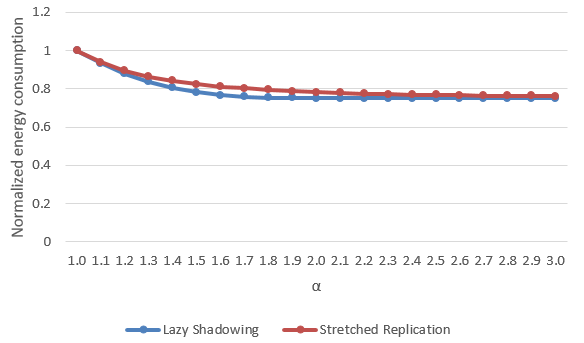
\includegraphics[width=\columnwidth]{figures/alpha_1.png}
		}
		\subfigure[$\rho=0.3$]
		{
			\label{fig:alpha_2}
			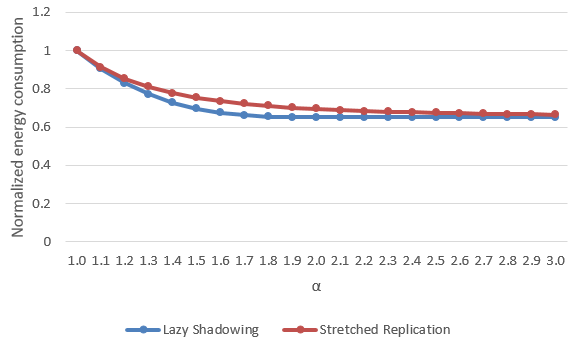
\includegraphics[width=\columnwidth]{figures/alpha_2.png}
		}
	\end{center}
	\caption{Normalized energy consumption for various response time laxities. W=240 hours, MTBF=5 years.}
	\label{fig:alpha}
\end{figure}


Figure~\ref{fig:alpha} shows that both lazy shadowing and stretched replication can achive over 20\% of energy savings compared to state machine repilcation, when there is enough laxity in the response time. When there is no laxity in the response time ($\alpha=1$), lazy shadowing and stretched replication don't have any freedom to reduce the execution rate of the shadow process, thus will execute both the main and shadow processes at the maximal execution rate, which essentially converges to state machine replication. In this case, it is staightforward that all three approaches have the same energy consumption. However, as laxity in response time increases, lazy shadowing and stretched replication immediately gain the ability to slow down the shadow process and thus save energy. It is also clear that laxy shadowing has more potential than stretched replication in energy saving. It can take better advantage of the laxity in respone time as it is more flexible in controling the execution rate than stretched replication. The highest difference is 4.5\% when $\alpha$ is around 1.5. As the laxity keeps increasing, the energy savings by lazy shadowing and stretched replication flatten out, as a result of the static power consumption. Since the static power consumption is independent of the execution rate, reducing the execution rate would extend the execution time, resulting in an increase in the energy consumption corresponding to the static power. Therefore, the minimal energy consumption would be achieved when there is a balance between energy from dynamic power and energy from static power, which may not be necessarily equivalent to using all the laxity in response time. It can be projected that if the staic power ratio is lower, laxy shadowing and stretched replication can take advantage of more laxity and achieve more energy saving compared to state machine replication. This will be discussed further in later section. At the right side of Figure~\ref{fig:alpha_1} and Figure~\ref{fig:alpha_2}, lazy shadowing and stretched replication converge when there is enough laxity for both of them. 

\subsection{Task vulnerability}
The objective of lazy shadowing is to minimize the expected energy consumption, considering the characteristics of both the task to execute and the underlying system. The probability of failure during the execution of the task is an important factor that will impact how the proposed fault tolerance approaches execute the task. Specifically, they will choose different process execution rates according to the likelyhood of failures. The ratio between the task workload and the MTBF is an approximation of the likelyhood of failure, assuming task workload is far less than the MTBF. In our experiments, we find that there is a linear relationship between task workload and MTBF in determining the optimal execution rates. Specifically, increasing the task workload has the same effect as decreasing the MTBF in our analytical models. Therefore, we combine them as a single parameter and refer to it as task vulnerability.

\begin{figure}[!t]	
	\begin{center}
		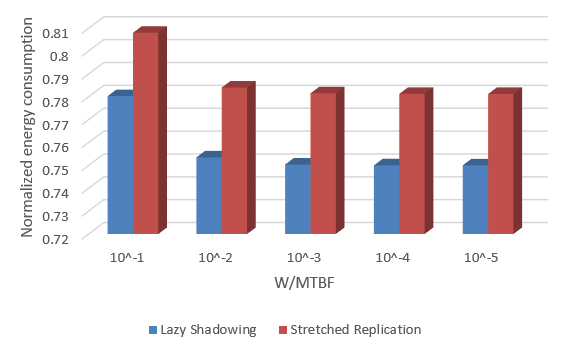
\includegraphics[width=\columnwidth]{figures/vulnerability.png}
	\end{center}
	\caption{Normalized energy consumption for various task vulnerabilities. $\rho$=0.5.}
	\label{fig:vulnerability}
\end{figure}

The results of the sensitivity study to task vulnerability, when $\rho=0.5$, are shown in Figure~\ref{fig:vulnerability}. From left to right, the task vulnerability decreases, meaning that the likelyhood of failure decreases. We can see that for all task vulnerabilities considered, both lazy shadowing and stretched replication can achieve significant energy savings over state machine replication. This indicates that the proposed approaches are scalable to future large-scale and failure-prone HPC environments. As task vulnerability decreases, lazy shadowing and stretched replication gains more energy savings. This is because the probability that the main process can complete the task without failure increases when task vulnerability decreases, increasing the probability that the shadow process can be terminated early to save energy. Again, lazy shadowing outperforms stretched replication because of its more flexibility in controling the execution rate of its shadow process.

\subsection{Static power ratio}
The computing nodes of each supercomputers have different power consumption characteristics, depending on the various computer organization and architecture technologies. Since our approaches are based on DVFS to control the process execution rates, the power consumption is partitioned into dynamic power, which has a superlinear relationship with the execution rate, and static power, which is unaffected by the execution rate. Static power ratio is an effecitve way to abstract the power saving ability of the proposed approaches on different machines.

\begin{figure}[!t]	
	\begin{center}
		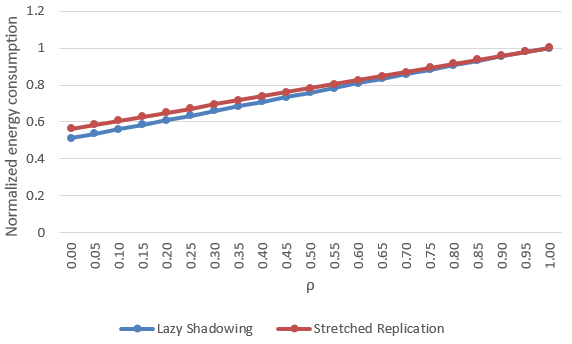
\includegraphics[width=\columnwidth]{figures/rho.png}
	\end{center}
	\caption{Normalized energy consumption for various static power ratios. W=240 hours, $\alpha$=2, MTBF=5 years.}
	\label{fig:rho}
\end{figure}

DVFS saves dynamic power while not changing static power. These two aspects have conflicting effects on the total energy consumption. By reducing the execution rate, the execution time increases proportionally. This also increases the energy consumption from static power proportionally as the static power is constant. However, since the dynamic power can be reduced superlinearly, the energy consumption corresponding to dynamic power is reduced, even though the execution is extended. The above analysis can be illustrated with Figure~\ref{fig:rho}. In addition, Figure~\ref{fig:rho} reveals that lazy shadowing can save up to 49\% of energy over state machine replication when consider dynamic power only. On the other hand, lazy shadowing and stretched replication are forced to execute both the main and shadow processes at the maximal rate when dynamic power is negligible, converging to the behavior of state machine replication. Current supercomputers have a static power ratio between 40\%-70\%, and it is reasonable to suspect that this will continue to be the case. Within this range, the energy saving is 14\%-29\% for lazy shadowing, and 13\%-26\% for stretched replication.



\section{Conclusion}
\label{conclusion}
%Current fault-tolerance approaches rely exclusively on either time or hardware redundancy for recovery. Rollback recovery  exploits time redundancy but can incur significant delay and high energy cost. On the other hand, process replication relies on hardware redundancy and requires a significant increase in resources and  power consumption.

In this paper, we propose Rejuvenating Shadows as a novel power-aware fault tolerance model, which guarantees forward progress, maintains consistent level of resilience, and minimizes implementation complexity and runtime overhead. Empirical experiments demonstrated that the Rejuvenating Shadows model outperforms in-memory checkpointing/restart in both execution time and resource utilization, especially in failure-prone environments.

Leaping induced by failure has proven to be critical in reducing the divergence between a main and its shadow, 
%with respect to workload execution.
%Consequently, the time to recover from subsequent failures is reduced significantly. 
thus reducing the recovery time for subsequent failures. Consequently, the time to recover from a failure increases with failure intervals.  
Based on this observation, a proactive approach is to ``force" leaping when the divergence between a main and its shadow exceeds a specified threshold. 
In our future work, we will further study this approach to determine what behavior triggers forced leaping in order to optimize the average recovery time. 

%we will study forcing the shadDuring experimentation we noticed the problem that recovery time in Rejuvenating Shadows can become substantial when the failure interval is large (Figure~\ref{fig:single_failure}). To deal with this issue, we are studying the idea of ``forced leaping", which borrows the idea from periodic checkpointing and forces a leaping whenever failure has been absent for a long time, in order to reduce the divergence between mains and shadows. Optimal intervals for forced leaping will be explored to balance between runtime overhead and failure recovery overhead. 

%In the future we plan to explore the integration with fault prediction techniques and the viability of dynamic and partial shadowing for platforms where nodes exhibit different ``health" status, e.g., some nodes may be more reliable while others are more likely to fail~\cite{gainaru2012fault}. 
%With this taken into account, we can apply dynamic scheduling of shadows only for mains that are likely to fail, to further reduce the resource requirement. 
%Another future direction is to study complier-assisted program slicing for fault detection. Specifically, slices that are fraction of their mains can run lazily as shadows and provide fault detection capability with reasonable coverage. 






%\begin{acknowledgements}
%If you'd like to thank anyone, place your comments here
%and remove the percent signs.
%\end{acknowledgements}

% BibTeX users please use one of
%\bibliographystyle{spbasic}      % basic style, author-year citations
\bibliographystyle{spmpsci}      % mathematics and physical sciences
%\bibliographystyle{spphys}       % APS-like style for physics
\bibliography{enahpc2015}   % name your BibTeX data base

% Non-BibTeX users please use
%\begin{thebibliography}{}
%
% and use \bibitem to create references. Consult the Instructions
% for authors for reference list style.
%
%\bibitem{RefJ}
% Format for Journal Reference
%Author, Article title, Journal, Volume, page numbers (year)
% Format for books
%\bibitem{RefB}
%Author, Book title, page numbers. Publisher, place (year)
% etc
%\end{thebibliography}

\end{document}
% end of file template.tex

